\chapter{Non-linear inequalities}
%\addcontentsline{toc}{chapter}{1 Graphs}
%%%%%%%%%%%%%%% SECTION HEADER %%%%%%%%%%%%%%%%
\rhead{3}
\lhead{Non-linear inequalities}
%%%%%%%%%%%%%%%%%%% START %%%$%%%%%%%%%%%%%%%%%
In chapter 1, we learned how to solve any linear inequalities plus absolute value inequalities. In this section, we will learn how to solve two types of non-linear inequalities:
\begin{enumerate}
    \item Polynomial inequality
    \item Rational inequality
\end{enumerate}
Before jumping to solve these types of inequalities, we begin the section by creating a sign table first.
% ======== SEC
\section{Sign table}
Of all functions we learned, linear function is the easiest one. Consider the linear function, $P(x) = x-3$. The first and easiest way to determine where the function is positive or negative, is \textbf{graphing}. The graph of this function is shown in Figure \ref{fig:boundary_point}.\\
\begin{figure}[ht]
    \centering
    \includegraphics[width=6cm]{pics/boundary_point.png}
    \caption{The graph of $P(x)=x-3$. Notice the boundary point is $3$}
    \label{fig:boundary_point}
\end{figure}


As you can see, point $x=3$ plays an important role; After this point, the graph is above the $x$-axis, therefore, it is positive. Whereas, before this point, the graph is below the $x$-axis and thus, it is negative. This point is called the \textit{boundary point} or \textit{critical point}.\\
The second method is the \textbf{algebraic method}. Since this method is much faster than first method, we will use this method instead of the first method. First, we need to find the boundary point by setting the function equal to 0, and then solving for $x$. In our example,
\begin{align*}
    P(x) &= 0 \\
    x-3 & = 0 \\
    x & =3 \qquad \text{Boundary point}
\end{align*}
Next, we draw a number line. The boundary point divide the whole number line into two intervals: $(-\infty,3)$ and $(3,+\infty)$. To find out the sign of $P(x)$, we choose one number within each intervals. You can choose any point you want, however, always try to choose a small number to make your calculation easy. Finally, plug each chosen number into $P(x)$ and see if you get a positive or negative value. If you get a positive value, that means the function $P(x)$ is always positive in that interval; Otherwise, it will be always negative.
\begin{table}[ht]
\centering
\begin{tabular}{c || c  c}
    \toprule
    Intervals     & $(-\infty,3)$   & $(3,+\infty)$\\[1.5pt]
    \hline \hline
    Chosen number & $0$         &  $4$ \\
    $P(x)$        & $P(0)=-3$  & $P(-3)=1$\\[1.5pt]
    Sign          &\circled{$-$} &\circled{$+$}
\end{tabular}
\end{table}


We can summarize all information we got in a number line shown in Figure \ref{fig:ST_ex} which is called the \textbf{sign table}.
% ==== FIGURE
\begin{figure}[ht]   
    \centering
    \begin{tikzpicture}[scale=0.7]
    \draw[->, thick] (-8,0) -- (8,0);
    \foreach \x in  {-7,...,7}
    \draw[shift={(\x,0)},color=black] (0pt,3pt) -- (0pt,-3pt);
    \foreach \x in {-7,...,7}
    \draw[shift={(\x,0)},color=black] (0pt,0pt) -- (0pt,-3pt) node[below] {$\x$};
    % Boundary point
    \draw (3,0) node[cross,red, ultra thick] {};
    %  Text above boundary point
    \node at (3,1) {Boundary point};
    \draw[->] (3,0.3) -- (3,0.7);
    % Signs
    \node at (-3,0.65) {\circled{$-$}};
    \node at (6,0.65) {\circled{$+$}};
    \end{tikzpicture}
    \caption{The sign table of $P(x)=x-3$.}
    \label{fig:ST_ex}
\end{figure}
% ====== NOTE
\begin{nt}
    In case of rational functions, we need to set both numerator and denominator equal to 0. Then solve them separately to find the boundary point(s). This is shown in the following example.
\end{nt}
% =======
\begin{exa}
    Create a sign table for the function $\displaystyle R(x) = \frac{x-5}{x+4}$.
\end{exa}
To find the boundary points, set numerator and denominator equal to 0.
\begin{align*}
        \text{Numerator}=0&       &       &\text{Denominator}=0 \\
        x-5 =0&                     &       &x+4=0\\
        x=5&                        &       &x=-4
\end{align*}    
So, we have two boundary points, $-4$ and $5$. These two points divide the whole number line into three sections: $(-\infty,-4)$, $(-4,5)$ and $(5,+\infty)$. We pick a number within each interval and plug them into $P(x)$ to find the sign of function in each interval.
\begin{table}[ht]
\centering
\begin{tabular}{c || c  c  c }
    \toprule
    Intervals     & $(-\infty,-4)$   & $(-4,5)$  & $(5,+\infty)$\\[1.5pt]
    \hline \hline
    Chosen number & $-5$         &  $-3$      &   $6$ \\
    $R(x)$        & $R(-5)=10$  & $R(-3)=-8$ & $R(6)=-1.25$ \\[1.5pt]
    Sign          &\circled{$+$} &\circled{$-$}&\circled{$+$}
\end{tabular}
\end{table}


The sign table of $R(x)$ is shown in Figure \ref{fig:ST_ex2} .
% ===== FIGURE
\begin{figure}[ht]   
    \centering
    \begin{tikzpicture}[scale=0.7]
    \draw[->, thick] (-8,0) -- (8,0);
    \foreach \x in  {-7,...,7}
    \draw[shift={(\x,0)},color=black] (0pt,3pt) -- (0pt,-3pt);
    \foreach \x in {-7,...,7}
    \draw[shift={(\x,0)},color=black] (0pt,0pt) -- (0pt,-3pt) node[below] {$\x$};
    % Boundary point
    \draw (-4,0) node[cross,red, ultra thick] {};
    \draw (5,0) node[cross,red, ultra thick] {};
    % Signs
    \node at (-7,0.65) {\circled{$+$}};
    \node at (0,0.65) {\circled{$-$}};
    \node at (7,0.65) {\circled{$+$}};
    \end{tikzpicture}
    \caption{The sign table of $R(x)=\frac{x-5}{x+4}$.}
    \label{fig:ST_ex2}
\end{figure}
% ======== 
\begin{tcolorbox}[title=Creating a sign table, 
                  fonttitle=\bfseries,
                  colframe=blue!75!black,
                  colback=blue!5!white]
Consider the function $F(x)$:
\begin{enumerate}[1.]
    \item \textbf{Boundary point(s)}: 
    \begin{itemize}
        \item If $F(x)$ is a polynomial, set it equal to 0 and solve for $x$.
        \item If $F(x)$ is a rational function, set both numerator and denominator equal to 0 and solve them separately. 
    \end{itemize}
    \item \textbf{Intervals:} The boundary point(s) divide(s) the number line into several intervals.
    \item \textbf{Pick a number}: choose a number withing each interval.Plug each chosen number into $F(x)$. 
    \begin{itemize}
        \item If $F(x)$ is positive, then the function is always positive within that interval.
        \item If $F(x)$ is negative, then the function is always negative within that interval.
    \end{itemize}
    \item \textbf{Sign}: Indicate the sign of each function withing each interval on the number line.
\end{enumerate}
\end{tcolorbox}
% ===== SEC
\section{Polynomial inequalities}
The first type of non-linear inequalities is polynomial inequalities. The first step to solve this inequality is to express it in the standard form, i.e. we must have a zero on one side :
\begin{align*}
            P(x) > 0 \qquad \text{or} \qquad P(x) < 0 \\
            \text{(same when we have $\le$ or $\ge$)}
\end{align*}
The next step, we find the boundary point(s) by solving $P(x)=0$. Then, we have to decide about boundary point(s): if we have $>$ or $<$, then the boundary points \underline{are not} included in our solution and we use open circle in our sign table. However, if we have $\ge$ or $\le$, then the boundary points are included and we use shaded circle in the sign table.\\
Once we completed our sign table, we look at the original inequalities and based on that we choose positive or negative intervals as our solution.
% =====
\begin{tcolorbox}[title=Solving a polynomial inequality,
                  fonttitle=\bfseries,
                  colframe=blue!75!black,
                  colback=blue!5!white]
    \begin{enumerate}[1.]
        \item \textbf{Standard form}: Express the equation in the standard form.
        \[
            P(x) <0 \quad or \quad P(x)>0 \quad  \text{(same for $\le$ or $\ge$)}
        \]
        \item \textbf{Sign table}: Create a sign table
        \item \textbf{Shaded or open circle}: We must decided whether the boundary points are included or excluded.
            \begin{itemize}
                \item For $<$ or $>$ $\longrightarrow$ excluded and use open circles.
                \item For $\le$ or $\ge$ $\longrightarrow$ included and use shaded circles.
            \end{itemize}
        \item \textbf{Choosing intervals}: Based on the original inequality, we can choose appropriate intervals:
            \begin{itemize}
                \item If $P(x)<0$ or $P(x) \le 0$ $\longrightarrow$ choose negative intervals.
                \item If $P(x)>0$ or $P(x) \ge 0$ $\longrightarrow$ choose positive intervals.
            \end{itemize}
    \end{enumerate}
\end{tcolorbox}
% ====== EXAMPLE
\begin{exa}
    Solve $x^2-4x<-3$
\end{exa}
First, add 3 to both sides to express the inequality in the standard form, $x^2-4x+3<0$. Let $P(x) = x^2-4x+3$. We must find the boundary points to create the sign table
\begin{align*}
        P(x) = 0&       &   &\text{Solve for $x$}\\
        x^2-4x+3=0&     &   &\text{Factor!}\\
        (x-1)(x-3)=0&   &   &\text{Set each factor equal to 0}\\
        x=1 \text{ or } x=3&  &   &\text{Our boundary points}
\end{align*}
These two points divide the number line into three sections:
\begin{table}[ht]
\centering
\begin{tabular}{c || c  c  c }
    \toprule
    Intervals     & $(-\infty,1)$   & $(1,3)$  & $(3,+\infty)$\\[1.5pt]
    \hline \hline
    Chosen number & $0$         &  $2$      &   $4$ \\
    $P(x)$        & $P(0)=3$  & $P(2)=-1$ & $P(4)=3$ \\[1.5pt]
    Sign          &\circled{$+$} &\circled{$-$}&\circled{$+$}
\end{tabular}
\end{table}


Since we have $<$ in our original inequality, therefore all boundary points are excluded and we use open circles.
\begin{figure}[ht]   
    \centering
    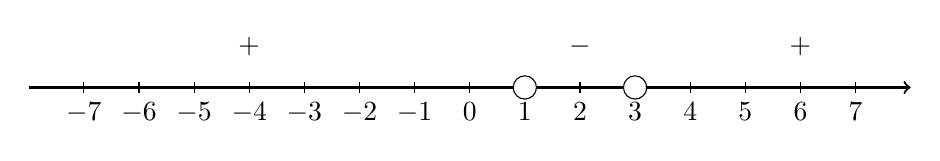
\begin{tikzpicture}[scale=0.7]
    \draw[->, thick] (-8,0) -- (8,0);
    \foreach \x in  {-7,...,7}
    \draw[shift={(\x,0)},color=black] (0pt,3pt) -- (0pt,-3pt);
    \foreach \x in {-7,...,7}
    \draw[shift={(\x,0)},color=black] (0pt,0pt) -- (0pt,-3pt) node[below] {$\x$};
    % Boundary point
    \fill[white] (1,0)  circle[radius=6pt]; 
    \draw (1,0)  circle[radius=6pt]; 
    \fill[white] (3,0)  circle[radius=6pt]; 
    \draw (3,0)  circle[radius=6pt]; 
    % Signs
    \node at (-4,0.75) {\circled{$+$}};
    \node at (2,0.75) {\circled{$-$}};
    \node at (6,0.75) {\circled{$+$}};
    \end{tikzpicture}
    \caption{The sign table of $P(x)=x^2-4x+3$.}
\end{figure}


Finally, we have $<$ in the original inequality, thus we should choose negative intervals. So our solution is $(-1,3)$. Notice $-1$ and $3$ are excluded.
% ======= EXAMPLE
\begin{exa}
    Solve $x^3-16x-x^2+16 \ge 0$
\end{exa}
The inequality is already in the standard form. Let $P(x)=x^3-16x-x^2+16$. So, we begin by finding the boundary points:
\begin{align*}
        P(x) = 0&       &   &\text{Solve for $x$}\\
        x^3-16x-x^2+16=0&     &   &\text{Factor $x$ from first two terms} \\
        &   &   &\text{and $-1$ from two last terms}\\
        x(x^2-16)-(x^2-16)=0&   &   &\text{Factor out $x^2-16$}\\
        (x^2-16)(x-1) =0&        &   &\text{Set each factor equal to 0}\\
        x=\pm 4 \text{  or } x=1&  &   &\text{Our boundary points}
\end{align*}
We have three boundary points dividing the number line into four intervals:
\begin{table}[ht]
\centering
\begin{tabular}{c || c  c  c  c }
    \toprule
    Intervals     & $(-\infty,-4)$   & $(-4,1)$  & $(1,4)$ & $(4,+\infty)$\\[1.5pt]
    \hline \hline
    Chosen number & $-5$         &  $0$      &   $2$   & $5$\\
    $P(x)$        & $P(-5)=-54$  & $P(0)=16$ & $P(2)=-12$ & $P(5)=36$\\[1.5pt]
    Sign          &\circled{$-$} &\circled{$+$}&\circled{$-$}&\circled{$+$}
\end{tabular}
\end{table}
%
\begin{figure}[ht]   
    \centering
    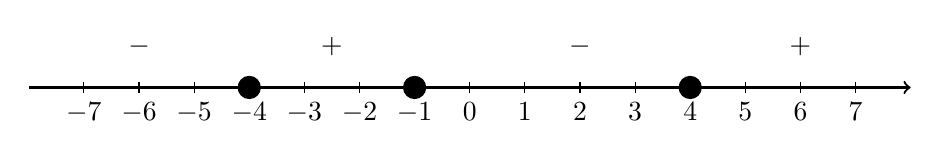
\begin{tikzpicture}[scale=0.7]
    \draw[->, thick] (-8,0) -- (8,0);
    \foreach \x in  {-7,...,7}
    \draw[shift={(\x,0)},color=black] (0pt,3pt) -- (0pt,-3pt);
    \foreach \x in {-7,...,7}
    \draw[shift={(\x,0)},color=black] (0pt,0pt) -- (0pt,-3pt) node[below] {$\x$};
    % Boundary point
    \fill[black] (-4,0)  circle[radius=6pt]; 
    \fill[black] (4,0)  circle[radius=6pt]; 
    \fill[black] (-1,0) circle[radius=6pt];
    % Signs
    \node at (-6,0.75) {\circled{$-$}};
    \node at (-2.5,0.75) {\circled{$+$}};
    \node at (2,0.75) {\circled{$-$}};
    \node at (6,0.75) {\circled{$+$}};
    \end{tikzpicture}
    \caption{The sign table of $P(x)=x^3-16x-x^2+16$.}
\end{figure}



Because of $\ge $ in the original inequality, all boundary points are included. Also we must choose, all positive intervals. So the solution is 
\[
            [-4,-1] \cup [4,+\infty)
\]
% ====== SEC
\section{Rational inequalities}
All steps are the same except the fact that zeros of denominator are always excluded. The zeros of numerator, however, depends on the inequality sign. If we have $<$ or $>$ then they are excluded; otherwise, they are included.
% =====
\begin{tcolorbox}[title=Solving a rational inequality, 
                  fonttitle=\bfseries,
                  colframe=blue!75!black,
                  colback=blue!5!white]
    \begin{enumerate}[1.]
        \item \textbf{Standard form}: Express the equation in the standard form.
        \[
            R(x) <0 \quad or \quad R(x)>0 \quad  \text{(same for $\le$ or $\ge$)}
        \]
        \item \textbf{Sign table}: Create a sign table
        \item \textbf{Shaded or open circle}: The boundary points of denominator are always excluded. For numerator:
            \begin{itemize}
                \item For $<$ or $>$ $\longrightarrow$ excluded and use open circles.
                \item For $\le$ or $\ge$ $\longrightarrow$ included and use shaded circles.
            \end{itemize}
        \item \textbf{Choosing intervals}: Based on the original inequality, we can choose appropriate intervals:
            \begin{itemize}
                \item If $R(x)<0$ or $R(x) \le 0$ $\longrightarrow$ choose negative intervals.
                \item If $R(x)>0$ or $R(x) \ge 0$ $\longrightarrow$ choose positive intervals.
            \end{itemize}
    \end{enumerate}
\end{tcolorbox}
% ====== EXAMPLE
\begin{exa}
    Solve $\frac{x-4}{(x-2)^2} \ge 0$
\end{exa}
The inequality is already expressed in standard form. Let $R(x)=\frac{x-4}{(x-2)^2}$ and find its boundary points
\begin{align*}
        \text{Numerator}=0&       &       &\text{Denominator}=0 \\
        x-4 =0&                     &       &(x-2)^2=0\\
        x=4&                        &       &x=2
\end{align*} 
These two boundary points will divide the number line into three intervals:
\begin{table}[ht]
\centering
\begin{tabular}{c || c  c  c }
    \toprule
    Intervals     & $(-\infty,2)$   & $(2,4)$  & $(4,+\infty)$\\[1.5pt]
    \hline \hline
    Chosen number & $1$         &  $3$      &   $5$\\
    $R(x)$        & $R(1)=-3$  & $R(3)=-1$ & $R(5)=0.11$\\[1.5pt]
    Sign          &\circled{$-$} &\circled{$-$}&\circled{$+$}
\end{tabular}
\end{table}
%

Notice, $x=2$ is a zero of denominator so it is excluded. $x=4$ is the zero of numerator and it's included because of $\ge$ in the original inequality.
%
\begin{figure}[ht]   
    \centering
    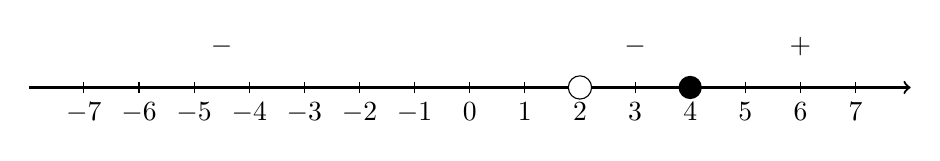
\begin{tikzpicture}[scale=0.7]
    \draw[->, thick] (-8,0) -- (8,0);
    \foreach \x in  {-7,...,7}
    \draw[shift={(\x,0)},color=black] (0pt,3pt) -- (0pt,-3pt);
    \foreach \x in {-7,...,7}
    \draw[shift={(\x,0)},color=black] (0pt,0pt) -- (0pt,-3pt) node[below] {$\x$};
    % Boundary point
    \fill[white] (2,0)  circle[radius=6pt];
    \draw (2,0)  circle[radius=6pt]; 
    \fill (4,0)  circle[radius=6pt]; 
    % Signs
    \node at (-4.5,0.75) {\circled{$-$}};
    \node at (3,0.75) {\circled{$-$}};
    \node at (6,0.75) {\circled{$+$}};
    \end{tikzpicture}
    \caption{The sign table of $R(x)=\frac{x-4}{(x-2)^2}$.}
\end{figure}
%


Because we have $\ge$ in the original inequality, we must select the positive signs. So our solution is $[4,+\infty)$.
% ========  EXAMPLE
\begin{exa}
    Solve $\frac{x-1}{x+3} < 1$
\end{exa}
First, we must express the inequality in the standard form. 
\begin{align*}
    \frac{x-1}{x+3} < 1&        &   &\text{Subtract 1}\\
    \frac{x-1}{x+3} -1<0&       &   &\text{LCD is $x+3$}\\
    \frac{x-1}{x+3} -1\biggl(\frac{x+3}{x+3}\biggr)<0&  &   &\text{Simplify}\\
    \frac{x-1-(x+3)}{x+3}<0&        &   &\text{Combine like terms}\\
    \frac{-4}{x+3} <0&      &       &\text{Standard form}
\end{align*}
Let $R(x) = \frac{-4}{x+3}$. Since we don't have any variable $x$ in numerator, so only set the denominator equal to 0.
\begin{align*}
    \text{Denominator} &= 0 \\
    x+3 &= 0\\
    x &= -3
\end{align*}
This boundary point divides the number line into two intervals.
%
\begin{table}[ht]
\centering
\begin{tabular}{c || c  c}
    \toprule
    Intervals     & $(-\infty,-3)$   & $(-3,+\infty)$\\[1.5pt]
    \hline \hline
    Chosen number & $-4$         &  $0$ \\
    $R(x)$        & $R(-4)=4$  & $R(-3)=-1.33$\\[1.5pt]
    Sign          &\circled{$+$} &\circled{$-$}
\end{tabular}
\end{table}
%

Don't forget $x=-3$ is the zero of the denominator thus, it is not included in our solution. Here is the sign table of $R(x)$:
\begin{figure}[ht]   
    \centering
    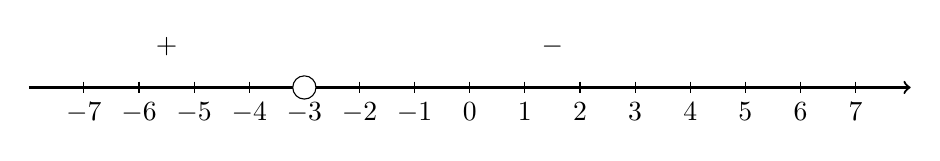
\begin{tikzpicture}[scale=0.7]
    \draw[->, thick] (-8,0) -- (8,0);
    \foreach \x in  {-7,...,7}
    \draw[shift={(\x,0)},color=black] (0pt,3pt) -- (0pt,-3pt);
    \foreach \x in {-7,...,7}
    \draw[shift={(\x,0)},color=black] (0pt,0pt) -- (0pt,-3pt) node[below] {$\x$};
    % Boundary point
    \fill[white] (-3,0)  circle[radius=6pt];
    \draw (-3,0)  circle[radius=6pt]; 
    % Signs
    \node at (-5.5,0.75) {\circled{$+$}};
    \node at (1.5,0.75) {\circled{$-$}};
    \end{tikzpicture}
    \caption{The sign table of $R(x)= \frac{-4}{x+3}$.}
\end{figure}
%

We have $<$ in the original inequality which means we are looking for negative intervals. Our solution is $(-3,+\infty)$.